\chapter{Results}
\label{chap:results}
\section{Bengio Style Curricula}
\label{chap:results:secBS}
As covered in our methodology section, we implemented the Corpus Replacement Simplification (CRS) curricula across the two sizes of wikitext datasets. We evaluate model performance on the validation portion at the end of each epoch, and once the model has trained for ten epochs, we evaluate using JIANT's \cite{Pruksachatkun2020jiantAS} implemented GLUE baseline. Unless another metric is explicitly mentioned, the GLUE sub-task metric is accuracy.
As seen in Figure \ref{fig:cs-perp-2} and Figure \ref{fig:cs-perp-103}, we see that the baseline method implementations outperform the CRS across the entire training regime in terms of validation perplexity. Initially, while the model is training on the limited corpus, it performs worse on the validation set. As the model reaches the original training data, the resulting embeddings reach close to the baseline perplexity but can never pass the baseline method. By the 7th epoch, both methods have virtually identical perplexities. Another interesting trend is that when the full corpus is introduced (epoch 6), the validation perplexity briefly increases. The final observation is that the baseline method reaches low perplexity on a large corpus much faster than the CRS method. The baseline method can achieve a perplexity under 100 by the end of the first epoch, while the CRS method cannot do so until the end of the 5th. \\
\begin{figure}[h]
\centering
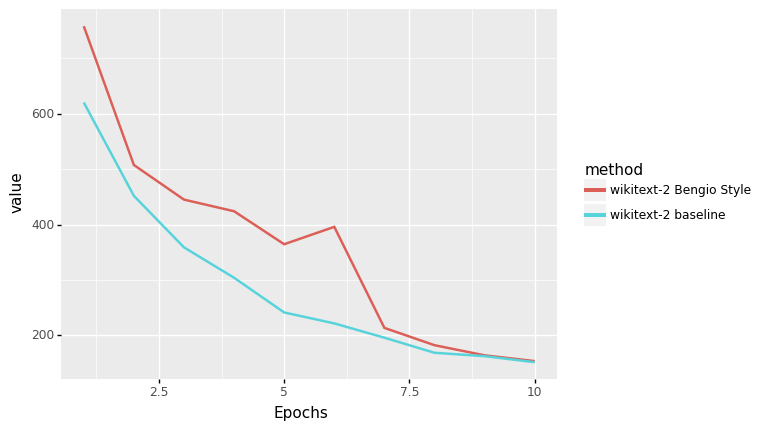
\includegraphics[width=10cm, height=10cm]{Thesis/images/wikitext-2BS.png}
\caption{Perplexity on Validation portion of wikitext2.}
\label{fig:cs-perp-2}
\end{figure}
\begin{figure}[h]
\centering
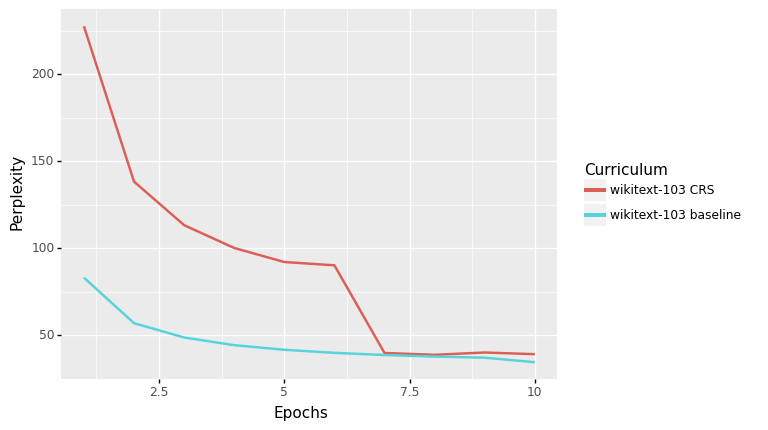
\includegraphics[width=15cm, height=10cm]{Thesis/images/wikitext-103BS.png}
\caption{Perplexity on Validation portion of wikitext103.}
\label{fig:cs-perp-103}
\end{figure}
\begin{table}[]
\begin{tabular}{|l|l|l|l|l|l|}
\hline
Method     & Baseline wiki103& CRS wiki103 & Baseline wiki2 & CRS wiki2 & Baseline BWC               \\ \hline \hline
\textbf{Overall Score}        & \textbf{0.671}        & 0.657        & 0.607      & 0.59       & 0.595                      \\ \hline
Cola(MCC)    & \textbf{0.281}        & 0.254        & 0.060       & 0.000          & 0.000                          \\ \hline
SST          & \textbf{0.862}        & 0.852        & 0.742      & 0.7        & 0.852                      \\ \hline
MRPC(F1)     & 0.866        & \textbf{0.875}        & 0.854      & 0.846      & 0.823                      \\ \hline
MRPC         & 0.801        & \textbf{0.816}        & 0.789      & 0.775      & 0.711                      \\ \hline
STS-B(Pear)  & 0.765        & \textbf{0.794}        & 0.683      & 0.661      & 0.547                      \\ \hline
STS-B(Spear) & 0.773        & \textbf{0.793}        & 0.684      & 0.663      & 0.562                      \\ \hline
QQP(F1)      & 0.716        & \textbf{0.738}        & 0.697      & 0.701      & 0.733                      \\ \hline
QQP          & 0.763        & \textbf{0.785}        & 0.745      & 0.753      & 0.765                      \\ \hline
MNLI         & 0.644        & 0.662        & 0.566      & 0.585      & \textbf{0.671}                      \\ \hline
QNLI         & \textbf{0.761}        & 0.719        & 0.726      & 0.717      & 0.719                      \\ \hline
RTE          & \textbf{0.610}         & 0.588        & 0.581      & 0.542      & 0.480                       \\ \hline
WNLI         & 0.535        & 0.437        & \textbf{0.563}      & \textbf{0.563}      & \textbf{0.563}                      \\ \hline
Diagnostic   & 0.139        & \textbf{0.162}        & 0.119      & 0.130       & 0.155 \\ \hline
\end{tabular}
\caption{GLUE results for CRS vs. baseline.}
\label{table:glue-corpus}
\end{table}
The effect of the curricula looking at GLUE can be found in Table \ref{table:glue-corpus} and we refer to the WikiText-103 corpus as wiki103, Wikitext-2 as wiki2 and the Billion Word Corpus as BWC. First, we find that the pubic ELMo implementation performs worse on the GLUE dataset. It is unclear why this is, and we will not focus on this further. Next, we see that when the training corpus is small, the BS implementation outperforms the baseline method by a sizable margin. As the corpus size grows, the baseline performance passes all other methods. There is high variability in individual task scores such that STS-B and the Diagnostic tests are much better with the BS system, while COLA, WNLI, and RTE are much better in the baseline method. One possible cause of this is BS models learn better representations for binary classifications but not better representations for multi-label classification. If we exclude WNLI, the BS methods outperform the baseline methods by a wide margin. We can also observe various tasks that the small corpus models cannot learn as both wikitext-2 models achieve 0 on COLA. We believe this may result from the model learning a flipped representation early on and not being able to recover from it. #Size of fine tuning datasets may be relevant
\section{Competence-Based Curricula}
Now we focus our discussion on the results of the competence curricula. In this section, DEP represents dependency parse depth, POS represents part of speech diversity, and CC represents competence curricula.
\subsection{Wikitext-2}
Looking at performance on the small corpus \fullref{fig:wikitext2-line-perplexity} and \fullref{fig:wikitext2-sentence-perplexity} we see that all the curricula methods start to overfit on the training corpus after about 16 of the 24 epochs (which equates to when the curriculum training is finished). The full data underpinning the figures mentioned above can be found in the \fullref{appendix}. Despite seeing over-fitting, we see that POS and DEP generally learn some of the lowest perplexity on the validation set. Looking at the difference between sentence-level and line-level training, we see a closer grouping in model performance distribution, which we attribute to a common sentence-level structure. Finally, we see that the best performance is achieved by the non-curricula baseline (initial competence set to 1) with a perplexity of 770, followed by Random with a perplexity of 2105. Despite the success of these curriculums, all are orders of magnitude above the baseline score of 151. We believe this failure of t #why is it so much worse\\
As we move our focus to GLUE results, we see a very different picture as the curriculum methods generally outperform the baselines by a wide margin. We see that models do not seem to learn any representation that can be used by WNLI, as those results are all virtually identical. Surprisingly it does not seem that a more optimal method for splitting the corpus is apparent as sentence-based training achieves a similar result in line-based training. We believe this means we cannot make a strong generalization that can be made about the effects of what method is used for training. The final point to observe is that nearly every curricula method outperforms the baseline implementation. Perhaps most surprising, random curricula performing second best when measure by overall glue score despite their being no motivation to the structure the model sees. \\
Overall when training on wikitext-2, we find that competency-based curricula methods provide somewhat of a mixed message. While performance on the validation portion is much worse, GLUE performance is much better. Since we believe what is most important in a model is how well the language representations can transfer to downstream tasks, we argue that with small training datasets CBC outperform traditional training regimes.

\begin{figure}[h]
\centering
\label{fig:wikitext2-line-perplexity}
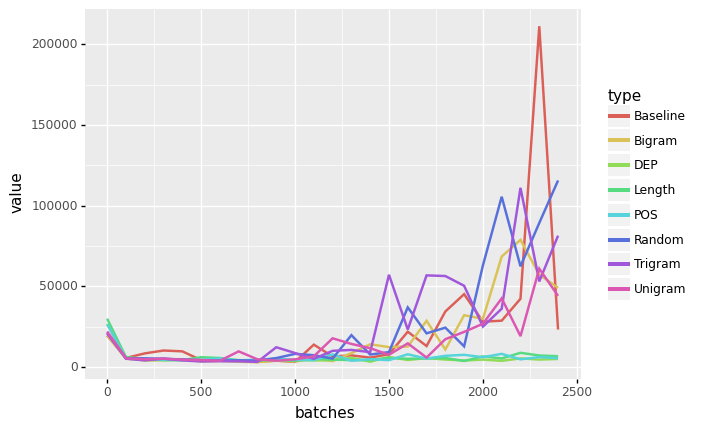
\includegraphics[width=10cm, height=10cm]{Thesis/images/wikitext-2line.png}
\caption{Model perplexity on wikitext2-line by curricula. DEP, POS, and LEN avoid the over-fitting the other models see}
\end{figure}



\begin{figure}[h]
\centering
\label{fig:wikitext2-sentence-perplexity}
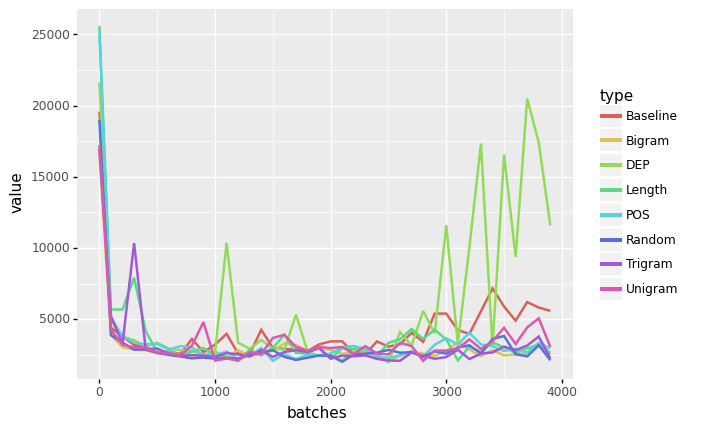
\includegraphics[width=10cm, height=10cm]{Thesis/images/wikitext-2sentence.png}
\caption{Model perplexity on wikitext2-sentence by curricula. Note DEP and trigram over fitting.}
\end{figure}

\begin{table}[h]
\begin{tabular}{|l|l|l|l|l|l|l|l|l|l|l|l|l|l|l|l|l|l|l}
\hline
Corpus       & sentence & sentence & sentence & sentence & sentence & line     & line     & line     & sentence & line     & line     & line     & line     & line     & line     & sentence & line     & sentence                   \\ \hline
Method       & cc       & cc       & cc       & cc       & cc       & cc       & cc       & cc       & cc       & cc       & cc       & cc       & cc       & bs       & cc       & cc       & baseline & cc                         \\ \hline
Curricula    & bigram   & random   & unigram  & POS      & DEP      & DEP      & unigram  & trigram  & trigram  & length   & baseline & bigram   & random   & N/A      & POS      & baseline & N/A      & length                     \\ \hline
Score        & 0.644556 & 0.643667 & 0.639833 & 0.637111 & 0.636    & 0.631944 & 0.628278 & 0.627444 & 0.626278 & 0.625444 & 0.621389 & 0.615833 & 0.614056 & 0.607111 & 0.606778 & 0.591056 & 0.589611 & 0.527889                   \\ \hline
Cola(MCC)    & 0.188    & 0.21     & 0.209    & 0.207    & 0.175    & 0.19     & 0.175    & 0.152    & 0.172    & 0.185    & 0.148    & 0.175    & 0        & 0.06     & 0        & 0.069    & 0        & -0.006                     \\ \hline
SST          & 0.79     & 0.78     & 0.755    & 0.765    & 0.792    & 0.727    & 0.768    & 0.761    & 0.788    & 0.748    & 0.747    & 0.768    & 0.763    & 0.742    & 0.737    & 0.768    & 0.7      & 0.75                       \\ \hline
MRPC(F1)     & 0.844    & 0.847    & 0.861    & 0.849    & 0.863    & 0.85     & 0.856    & 0.838    & 0.833    & 0.844    & 0.836    & 0.856    & 0.847    & 0.854    & 0.842    & 0.847    & 0.846    & 0.805                      \\ \hline
MRPC         & 0.775    & 0.779    & 0.799    & 0.777    & 0.797    & 0.782    & 0.782    & 0.762    & 0.779    & 0.77     & 0.77     & 0.782    & 0.775    & 0.789    & 0.77     & 0.765    & 0.775    & 0.674                      \\ \hline
STS-B(Pear)  & 0.732    & 0.715    & 0.731    & 0.714    & 0.721    & 0.708    & 0.675    & 0.695    & 0.73     & 0.658    & 0.706    & 0.675    & 0.699    & 0.683    & 0.663    & 0.728    & 0.661    & 0.708                      \\ \hline
STS-B(Spear) & 0.733    & 0.712    & 0.731    & 0.714    & 0.72     & 0.704    & 0.674    & 0.691    & 0.731    & 0.654    & 0.705    & 0.674    & 0.699    & 0.684    & 0.66     & 0.731    & 0.663    & 0.71                       \\ \hline
QQP(F1)      & 0.742    & 0.744    & 0.733    & 0.727    & 0.727    & 0.735    & 0.738    & 0.73     & 0.744    & 0.725    & 0.734    & 0.738    & 0.721    & 0.697    & 0.712    & 0.722    & 0.701    & 0.537                      \\ \hline
QQP          & 0.788    & 0.791    & 0.778    & 0.781    & 0.786    & 0.782    & 0.792    & 0.782    & 0.796    & 0.783    & 0.78     & 0.792    & 0.784    & 0.745    & 0.771    & 0.758    & 0.753    & 0.682                      \\ \hline
MNLI         & 0.617    & 0.616    & 0.613    & 0.606    & 0.613    & 0.598    & 0.598    & 0.616    & 0.62     & 0.601    & 0.612    & 0.598    & 0.611    & 0.566    & 0.61     & 0.5      & 0.585    & 0.326                      \\ \hline
QNLI         & 0.766    & 0.76     & 0.757    & 0.745    & 0.749    & 0.748    & 0.746    & 0.764    & 0.761    & 0.748    & 0.719    & 0.746    & 0.749    & 0.726    & 0.75     & 0.718    & 0.717    & 0.51                       \\ \hline
RTE          & 0.57     & 0.57     & 0.545    & 0.567    & 0.567    & 0.581    & 0.56     & 0.542    & 0.552    & 0.567    & 0.538    & 0.56     & 0.578    & 0.581    & 0.592    & 0.538    & 0.542    & 0.592                      \\ \hline
WNLI         & 0.563    & 0.563    & 0.563    & 0.563    & 0.521    & 0.563    & 0.549    & 0.563    & 0.437    & 0.563    & 0.563    & 0.437    & 0.563    & 0.563    & 0.563    & 0.451    & 0.563    & 0.521                      \\ \hline
Diagnostic   & 0.131    & 0.143    & 0.135    & 0.134    & 0.137    & 0.118    & 0.132    & 0.144    & 0.137    & 0.128    & 0.121    & 0.132    & 0.143    & 0.119    & 0.155    & 0.107    & 0.13     & \multicolumn{1}{l|}{0.008}
\end{tabular}
\caption{GLUE results for BS vs baseline.\\ Model performance is better with BS when corpus is small but as corpus scales baseline method out performs BS}
\label{tab:wiki2-glue}
\end{table}

\subsection{wikitext-103}
As we scale to the larger corpus, we find that not all the small data hold trends. Looking at the results in \fullref{fig:wikitext-103-line} and \fullref{fig:wikitext-103-sentence}, we can see that similar to the smaller corpus, none of the curriculums learned methods can learn a representation that transfers well to the validation set. We have removed the baseline and the N-gram methods from the line chart as they made understanding model performance difficult. Complete tables are available in \fullref{appendix}. Unlike the non-curricula techniques, which achieve a perplexity of 36, none of the curricula methods ever learn a model with a perplexity under one thousand. We note that similar to what was seen on the wikitext-2 is on wikitext-103. N-gram methods have a similar distribution in performance. Also, holding over from wikitext-2, DEP, LEN, and POS demonstrates a slow and steady improvement in perplexity as their training continues. As the dataset has grown larger, we see increased volatility in perplexity changes across all training methods.\\
Looking at the result of the transfer tasks as measured by GLUE \ref{glue-wiki-103}, we find that the trends we see in the smaller corpus no longer hold. The best model in terms of transfer learning is the non-curriculum baseline implementation from the original ELMo implementation. This baseline method outperforms on the overall score and outperforms every other model on tasks like CoLA, where the score is nearly 20\% better. Surprisingly, after the baseline method, the trigram curricula appear to generate the best transfer task as both sentence and line-based methods as they are ranked second and third when measured on the average across tasks. We also note that some of the best performing curricula are also those models that had some of the highest perplexities on the training task.

\begin{table}[]
\centering
\resizebox{\textwidth}{!}{%
\begin{tabular}{|l|l|l|l|l|l|l|l|l|l|l|l|l|l|l|l|l|}
\hline
Corpus style & Train Method & Competence Method & Score & Cola(MCC) & SST & MRPC(F1) & MRPC & STS-B(Pear) & STS-B(Spear) & QQP(F1) & QQP & MNLI & QNLI & RTE & WNLI & Diagnostic \\ \hline
line & baseline & N/A & 0.670556 & 0.281 & 0.862 & 0.866 & 0.801 & 0.765 & 0.773 & 0.716 & 0.763 & 0.644 & 0.761 & 0.61 & 0.535 & 0.139 \\ \hline
sentence & Competence Curriculum & trigram & 0.665722 & 0.208 & 0.857 & 0.865 & 0.806 & 0.79 & 0.79 & 0.733 & 0.779 & 0.658 & 0.757 & 0.567 & 0.563 & 0.136 \\ \hline
line & Competence Curriculum & trigram & 0.664722 & 0.207 & 0.854 & 0.871 & 0.804 & 0.781 & 0.782 & 0.752 & 0.799 & 0.655 & 0.767 & 0.556 & 0.549 & 0.144 \\ \hline
sentence & Competence Curriculum & unigram & 0.663778 & 0.19 & 0.856 & 0.861 & 0.797 & 0.784 & 0.784 & 0.747 & 0.791 & 0.654 & 0.773 & 0.556 & 0.563 & 0.14 \\ \hline
sentence & Competence Curriculum & baseline & 0.663278 & 0.19 & 0.845 & 0.878 & 0.824 & 0.767 & 0.768 & 0.748 & 0.788 & 0.651 & 0.746 & 0.588 & 0.563 & 0.14 \\ \hline
line & Competence Curriculum & baseline & 0.663056 & 0.214 & 0.826 & 0.865 & 0.804 & 0.766 & 0.766 & 0.747 & 0.789 & 0.643 & 0.772 & 0.581 & 0.563 & 0.145 \\ \hline
sentence & Competence Curriculum & random & 0.661444 & 0.203 & 0.843 & 0.87 & 0.806 & 0.778 & 0.779 & 0.74 & 0.789 & 0.644 & 0.745 & 0.574 & 0.563 & 0.151 \\ \hline
sentence & Competence Curriculum & length & 0.658556 & 0.229 & 0.827 & 0.867 & 0.804 & 0.765 & 0.766 & 0.747 & 0.783 & 0.642 & 0.762 & 0.538 & 0.563 & 0.135 \\ \hline
line & Bengio curricula & N/A & 0.656944 & 0.254 & 0.852 & 0.875 & 0.816 & 0.794 & 0.793 & 0.738 & 0.785 & 0.662 & 0.719 & 0.588 & 0.437 & 0.162 \\
line & Competence Curriculum & bigram & 0.656278 & 0.18 & 0.826 & 0.854 & 0.792 & 0.77 & 0.77 & 0.753 & 0.794 & 0.645 & 0.766 & 0.56 & 0.563 & 0.137 \\
line & Competence Curriculum & length & 0.656 & 0.212 & 0.82 & 0.851 & 0.782 & 0.768 & 0.767 & 0.734 & 0.788 & 0.634 & 0.752 & 0.578 & 0.563 & 0.135 \\ \hline
line & Competence Curriculum & unigram & 0.653611 & 0.194 & 0.823 & 0.857 & 0.789 & 0.755 & 0.754 & 0.752 & 0.794 & 0.625 & 0.753 & 0.574 & 0.563 & 0.125 \\ \hline
line & Competence Curriculum & random & 0.652333 & 0.179 & 0.836 & 0.861 & 0.789 & 0.772 & 0.774 & 0.753 & 0.797 & 0.64 & 0.772 & 0.578 & 0.493 & 0.139 \\ \hline
line & Competence Curriculum & part of speech diversity & 0.649056 & 0.163 & 0.827 & 0.861 & 0.794 & 0.756 & 0.757 & 0.754 & 0.791 & 0.63 & 0.732 & 0.57 & 0.563 & 0.138 \\ \hline
sentence & Competence Curriculum & bigram & 0.648611 & 0.195 & 0.859 & 0.867 & 0.799 & 0.784 & 0.785 & 0.736 & 0.772 & 0.651 & 0.754 & 0.599 & 0.408 & 0.132 \\ \hline
line & Competence Curriculum & dependency parse depth & 0.644389 & 0.231 & 0.846 & 0.856 & 0.779 & 0.776 & 0.776 & 0.746 & 0.786 & 0.637 & 0.761 & 0.542 & 0.423 & 0.137 \\ \hline
sentence & Competence Curriculum & part of speech diversity & 0.639889 & 0.114 & 0.794 & 0.853 & 0.772 & 0.775 & 0.774 & 0.74 & 0.782 & 0.624 & 0.738 & 0.578 & 0.563 & 0.108 \\ \hline
sentence & Competence Curriculum & dependency parse depth & 0.5865 & -0.04 & 0.842 & 0.805 & 0.679 & 0.786 & 0.789 & 0.682 & 0.73 & 0.321 & 0.757 & 0.614 & 0.549 & 0.038 \\ \hline
\end{tabular}
}
\caption{GLUE performance on models trained with wikitext-103}
\label{tab:glue-wiki-103}
\end{table}
\begin{figure}[h]
\centering
\label{fig:wikitext-103-line}
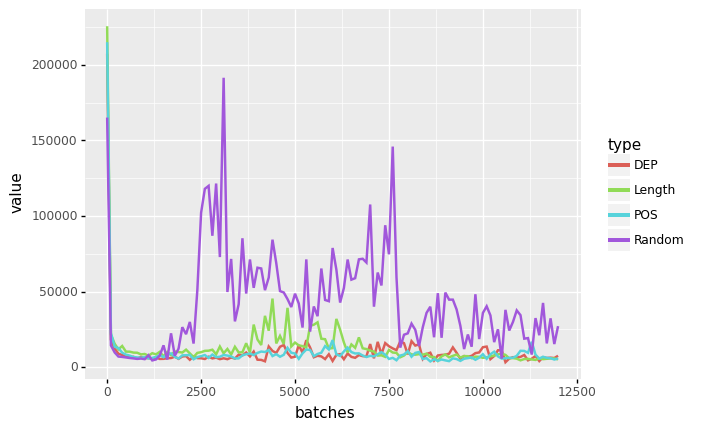
\includegraphics[width=10cm, height=10cm]{Thesis/images/wikitext-103lineminusbigrambaselinetrigramunigram.png}
\caption{Model perplexity on wikitext103-line by curricula. N-gram methods and Baseline have been removed to allow easier interpretation.}
\end{figure}
\begin{figure}[h]
\centering
\label{fig:wikitext-103-sentence}
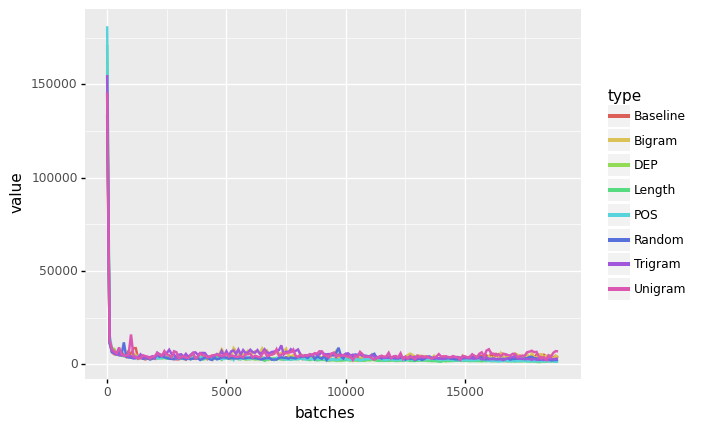
\includegraphics[width=10cm, height=10cm]{Thesis/images/wikitext-103sentenceraw.png}
\caption{Model perplexity on wikitext103-sentence by curricula.}
\end{figure}
\section{Discussion}
We find it useful to formulate CL as moving from sampling without replacement to sampling with replacement with an ever-growing population. As a result, our implementations of CBC do not guarantee that the model will see the entire dataset ten times, and as a result, the distribution of the data seen in training is likely different from the distribution of the validation dataset. We believe this is why the CL implementations can never generalize their performance in the train portion of the corpus to the validation portion. To avoid this one such approach would be to over sample easy portions of the training data in early training and extend the length of this epoch. This way the model could build of easy example but still see every part of the training corpus at least ten times. \\
Despite this inability to learn the training distribution, CBC methods are still able to transfer well to understanding tasks, which makes us think that what is important in pre-training is not the actual task but what the model can learn from the task. This finding is interesting because it challenges the notion that a model must fit the target dataset well to learn a representation that transfers well to downstream tasks. We find that even the models with high validation perplexities can still learn good representations for our transfer task. \\
Another observation our data leads us to is how the training distribution's tweaking can allow the models to do better in transfer tasks because it is unable to overfit to the small pre-training corpus. Since our implementation generates some form of continually changing data distribution from where random batches are sampled, the train distribution is continually changing. Since the training regime is constantly changing, we CBC is effectively simulating a larger, more complex distribution. On one hand, this larger artificial training set causes the model never learns a good representation of the training corpus which we see in model perplexity. On the other hand, since it never learns a good representation of the training corpus it can effectively simulate a much larger training corpus which produces a LR which when measured in terms of transfer performance is much better. This is especially apparent in the effectiveness of random curricula, where the random training structure still leads to improved transfer performance. Instead of having one consistent dataset of size $N$ we have a dataset of $size = \sum_{t=0} N * \lambda_t$ datasets.  \\
Independently of what heuristic is used in early training, some portion (usually the easy portion) is oversampled while in other portions (usually hard portion), examples are under-sampled. Recently, work in understanding how NN work has lead to the discovery there are sub-networks within the larger NN, which are more optimal for the task \cite{Frankle2019TheLT}. The process of training a DNN can be thought of as an architecture search within the larger randomly initiated network by decreasing the weights of sub-optimal sub-networks and increasing the weights of optimal sub-networks. Since the CL method is oversampling some portion of the dataset during early training, CL methods will favor sub-networks that are likely not optimal for the full data distribution. We believe this may be the cause of why CL methods underperform non-CL methods on the training task. One way to address this shortcoming would be to modify curricula methods to create ever-changing distributions that are close to the original distribution. In other words, in early training, instead of oversampling from the lower strata of the CDF CL methods could sample from slightly distorted distributions of the same CDF. One such implementation may divide the data into deciles and sample from each decile for each epoch. In other words instead of sampling from the whole distribution the first training epoch would sample from the lowest 10\% of the CDF while the last training epoch would sample from the highest 10\%. \\ 
An additional observation more focused on LM training is there is no marked difference in the effects of training with sentence-based corpora vs. that of line-based datasets. This, matched with no generalized Superior curricula performance, heuristic makes us believe that language models learn more from the random distribution of a textual corpus than any structure experimenters try to introduce. Our experiments, in many ways, show how robust and efficient regular stochastic sampling is. The cost of shuffling happens once instead of every batch, and no additional work needs to go to crafting the curricula.\\
With regard to improving the efficiency of LM training unfortunately our models had the opposite effect. Our implementation of CBC introduces an overhead which makes training over 40\% less efficient. In seeing the effective impact of successful training datasets like the Toronto Book corpus we believe that successful CL methods need to focus on rebalancing training distribution in a model independent method. By rebalancing data distributions CL methods can ensure that the cost of compute only happens once instead of the $n$ times the data is resampled in model training and the $m$  potential models that use this data. Moreover, by moving curriculum generation outside of model training CL methods can have a larger impact because researchers only need to train on a new dataset instead of changing their model code. \\
When we focus on the difference between sentence based sampling vs line based sampling we find a huge difference in model performance on the validation corpus but no noticeable difference in the GLUE. In evaluating the data we believe this is caused by the inefficiency introduced by our padding token. Since sentence based sampling has ~30\% more padding tokens the model is able to learn substantially less from every sample when compared to the line corpus. This greatly effects the models ability to learn the training distribution but does not have any generalizable impact on the transfer performance. This is in line with the purpose of pretraining as the goal is not actually to learn the training data but use it to form a generalizable understanding based on a lose connection. As a result being unable to fully learn the training distribution does not seem to effect the learned signal that is transferred. \\
Reflecting on our experiments and questions posed earlier in the dissertation in Section \ref{chap:method}:
\begin{enumerate}
\item CL can help converge to a more optimal global minima when the training corpus is small. As corpus size scales, the positive impact of CL disappears.
\item The downstream representation learned via CL outperforms non-curricula methods when the corpus size is small, but as the corpus size grows, CL methods no longer generate the best representation.
\item CL methods do not help the model convergence speed in any noticeable way and in our use of padding tokens CL methods actually make training fare less efficient than non CL methods.
\end{enumerate}